\documentclass[9pt]{beamer}
\usetheme{Antibes}
\useinnertheme{rectangles}
\useoutertheme{infolines}
\usepackage[utf8]{inputenc}
\usepackage[T1]{fontenc}
\usepackage[ngerman]{babel}

% patch the look of +, = in arev
\usefonttheme{serif} 

\usepackage{arev}
\usepackage{amsmath}
\usepackage{amssymb}

\setbeamertemplate{footline}{%
\begin{beamercolorbox}[ht=3.0ex,dp=1ex]{title in head/foot}
\hfill\footnotesize\insertpagenumber\enspace\enspace\end{beamercolorbox}}

\definecolor{bluegreen1}{rgb}{0.0,0.20,0.28}
\definecolor{bluegreen2}{rgb}{0.0,0.20,0.28}
\setbeamercolor*{palette primary}{fg=white,bg=bluegreen1}
\setbeamercolor*{palette secondary}{fg=white,bg=bluegreen2}
\setbeamercolor*{palette tertiary}{fg=white,bg=bluegreen2}
\setbeamercolor{itemize item}{fg=black}
\setbeamercolor{block title}{bg=bluegreen2}
\newcommand{\modest}[1]{{\small\color{gray}#1}}

\newcommand{\ee}{\mathrm e}
\newcommand{\ui}{\mathrm i}
\newcommand{\real}{\operatorname{Re}}
\newcommand{\imag}{\operatorname{Im}}
\newcommand{\uv}[1]{\underline{#1}}
\newcommand{\bv}[1]{\mathbf{#1}}

\newcommand{\N}{\mathbb N}
\newcommand{\Z}{\mathbb Z}
\newcommand{\Q}{\mathbb Q}
\newcommand{\R}{\mathbb R}
\newcommand{\C}{\mathbb C}

\newcommand{\id}{\operatorname{id}}
\newcommand{\sgn}{\operatorname{sgn}}
\newcommand{\Abb}{\operatorname{Abb}}
\newcommand{\unit}[1]{\mathrm{#1}}
\newcommand{\chem}[1]{\mathrm{#1}}
\newcommand{\strong}[1]{\textsf{\textbf{#1}}}
\newcommand{\defiff}{\quad:\Longleftrightarrow\quad}

\newcommand{\icol}[1]{
  \big(\!\begin{smallmatrix}#1\end{smallmatrix}\!\big)%
}

\newcommand{\parspace}{\vspace{0.8em}}


\title{Was ist ein Basiswechsel?}
\date{}

\begin{document}

\begin{frame}
\maketitle
\end{frame}

\begin{frame}[t]
\vspace{3em}
Betrachten wir einen Vektor $\bv v$ im Koordinatenraum $\R^2$.

\parspace
Z.\,B. $\bv v:=\icol{9\\ 5}$.\pause

\vspace{-1em}
\begin{center}
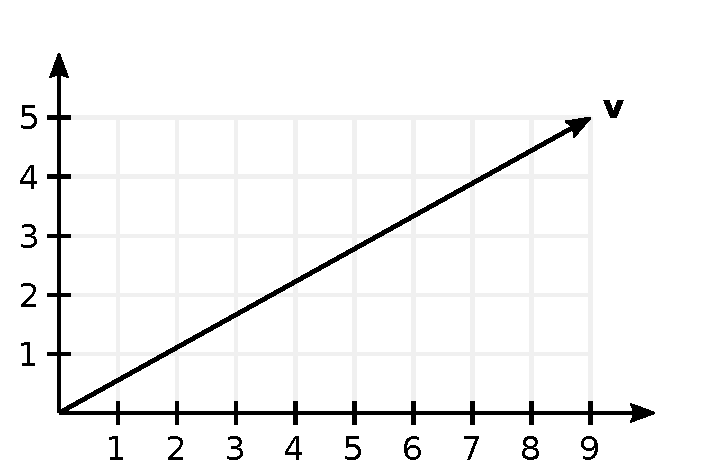
\includegraphics[width=72mm]{img/Vektor.pdf}
\end{center}
\end{frame}

\begin{frame}[t]
\vspace{3em}
Bezüglich einer Basis $B=(\bv b_1,\bv b_2)$ besitzt der
Vektor eine andere Darstellung.\pause

\vspace{0.8em}
Sei z.\,B. $\bv b_1 := \icol{4\\ 1}$ und $\bv b_2 := \icol{1\\ 3}$.%
\pause

\vspace{-1.6em}
\begin{center}
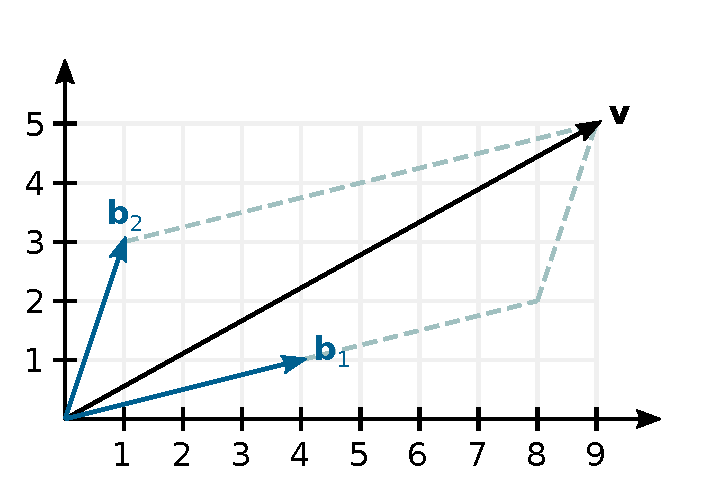
\includegraphics[width=72mm]{img/Vektor-in-Basis-B.pdf}
\end{center}
\end{frame}

\begin{frame}[t]
\vspace{4em}
Bezüglich $B$ besitzt der Vektor die Darstellung
\[\bv v = 2\bv b_1 + 1\bv b_2 = x'\bv b_1 + y'\bv b_2.
\]\pause
Das Tupel $\bv v_B = (x',y')$ nennen wir \emph{Koordinatenvektor}
zum Vektor $\bv v$ bezüglich Basis $B$.\pause

\parspace
Angenommen, es gibt nun noch eine weitere Basis $A=(\bv a_1,\bv a_2)$.\\
Z.\,B. $\bv a_1:=\icol{7\\ 1}$ und $\bv a_2:=\icol{1\\ 2}$.\pause

\vspace{1.2em}
Wie findet man dann den Koordinatenvektor $\bv v_A=(x,y)$ mit
\[\bv v = x\bv a_1 + y\bv a_2?\]
\end{frame}

\begin{frame}
\begin{center}
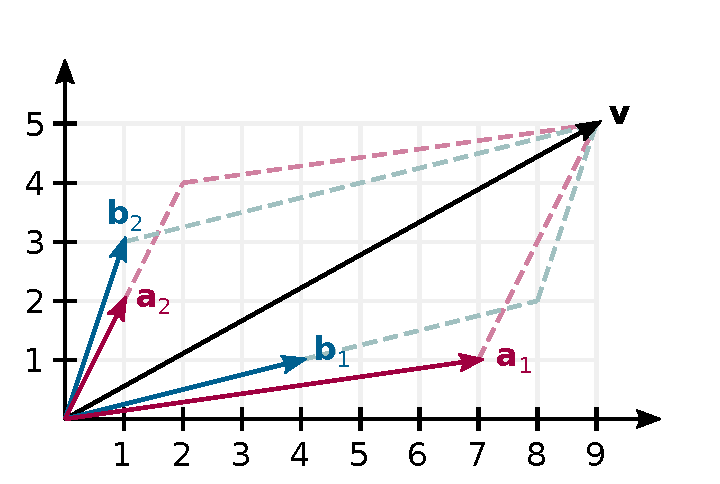
\includegraphics[width=72mm]{img/Vektor-in-Basis-BA.pdf}
\end{center}
\end{frame}

\begin{frame}[t]
\vspace{4em}
Trick: Wir ordnen der Basis
$A=(\begin{pmatrix}a_{11}\\ a_{21}\end{pmatrix},
\begin{pmatrix}a_{12}\\ a_{22}\end{pmatrix})$
die Matrix
\[A=\begin{pmatrix}a_{11} & a_{12}\\ a_{21} & a_{22}\end{pmatrix}\]
zu.\pause{} Dann gilt nämlich
\begin{align*}
\bv v &= x\bv a_1 + y\bv a_2 = x\begin{pmatrix}a_{11}\\ a_{21}\end{pmatrix}
+ y\begin{pmatrix}a_{12}\\ a_{22}\end{pmatrix}\\
&= \begin{pmatrix}a_{11}x + a_{12}y\\ a_{21}x + a_{22}y\end{pmatrix}
= \begin{pmatrix}a_{11} & a_{12}\\ a_{21} & a_{22}\end{pmatrix}\begin{pmatrix}x\\ y\end{pmatrix}
= A\bv v_A.
\end{align*}
\end{frame}

\begin{frame}
Für die Basis $B$ gilt die gleiche Überlegung. Daher ist
\[\bv v = A\bv v_A = B\bv v_B.\]\pause
Weil $A$ eine Basis ist, ist $\det(A)\ne 0$, womit $A$ eine
inverse Matrix $A^{-1}$ besitzt. Multiplizieren wir beide Seiten
der Gleichung von links mit $A^{-1}$, bekommen wir
\[\bv v_A = E\bv v_A = A^{-1}A\bv v_A = A^{-1}B\bv v_B.\]
Das ist der gesuchte Koordinatenvektor.
\end{frame}

\begin{frame}
Anders ausgedrückt ist $A\bv v_A = B\bv v_B$ ein lineares
Gleichungssystem in $\bv v_A=(x,y)$.\pause{} Das ist
\[\begin{pmatrix}a_{11} & a_{12}\\ a_{21} & a_{22}\end{pmatrix}\begin{pmatrix}x\\ y\end{pmatrix}
= \begin{pmatrix}b_{11} & b_{12}\\ b_{21} & b_{22}\end{pmatrix}\begin{pmatrix}x'\\ y'\end{pmatrix}.
\]\pause{}
Im Beispiel ist
\[\begin{pmatrix}7 & 1\\ 1 & 2\end{pmatrix}\begin{pmatrix}x\\ y\end{pmatrix}
= \begin{pmatrix}4 & 1\\ 1 & 3\end{pmatrix}\begin{pmatrix}2\\ 1\end{pmatrix}
= \begin{pmatrix}9\\ 5\end{pmatrix}.\]\pause
Das macht $x=1$ und $y=2$.
\end{frame}

\begin{frame}
Woher ist eigentlich die Darstellung $\bv v_A$ bekannt?\pause

\vspace{0.8em}
Die bekommen wir auf die gleiche Art.  Die Gleichung
\[\bv v = B\bv v_B\]
müssen wir dazu bloß nach $\bv v_B$ umformen. D.\,h.
$\bv v_B = B^{-1}\bv v$.\pause

\vspace{0.8em}
Bzw. es liegt ein lineares Gleichungssystem
in $\bv v_B$ vor.
\end{frame}

\begin{frame}
\strong{Bemerkung.} Man beachte
\[\bv v = \begin{pmatrix}9\\ 5\end{pmatrix} = 
9\begin{pmatrix}1\\ 0\end{pmatrix} + 5\begin{pmatrix}0\\ 1\end{pmatrix}
= 9\bv e_1 + 5\bv e_2.\]\pause
Die Matrix zur Standardbasis $(\bv e_1,\bv e_2)$
ist die Einheitsmatrix
\[E=\begin{pmatrix}1 & 0\\ 0 & 1\end{pmatrix}.
\]\pause
Daher gilt $\bv v = E\bv v_E = \bv v_E$. D.\,h. ein Koordinatenvektor
ist sein eigener Koordinatenvektor. 
\end{frame}

\begin{frame}
\begin{center}
\strong{Kurze Pause}
\end{center}
\end{frame}

\begin{frame}
Nun tauschen wir $\R^2$ gegen einen abstrakten Vektorraum $V$ aus.
Damit ist gemeint, dass nun nicht mehr a priori ein absolutes
Koordinatensystem vorliegt.\pause

\vspace{0.8em}
Dies zieht einige Konsequenzen nach sich. Zum einen existiert für
$\bv v$ keine absolute Darstellung mehr. Zudem sind auch die
Basisvektoren davon betroffen.\pause

\vspace{0.8em}
Da die Matrizen $A$ und $B$ jeweils aus der absoluten Darstellung
ihrer Basisvektoren aufgebaut sind, existieren auch diese nicht mehr.
\end{frame}

\begin{frame}
\begin{center}Vektorraum $\R^2$\end{center}

\vspace{-2em}
\begin{center}
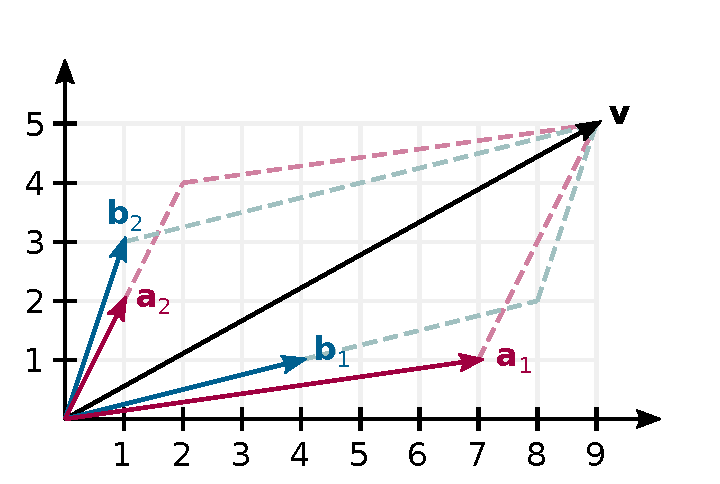
\includegraphics[width=72mm]{img/Vektor-in-Basis-BA.pdf}
\end{center}
\end{frame}

\begin{frame}
\begin{center}Vektorraum $V$\end{center}

\vspace{-2em}
\begin{center}
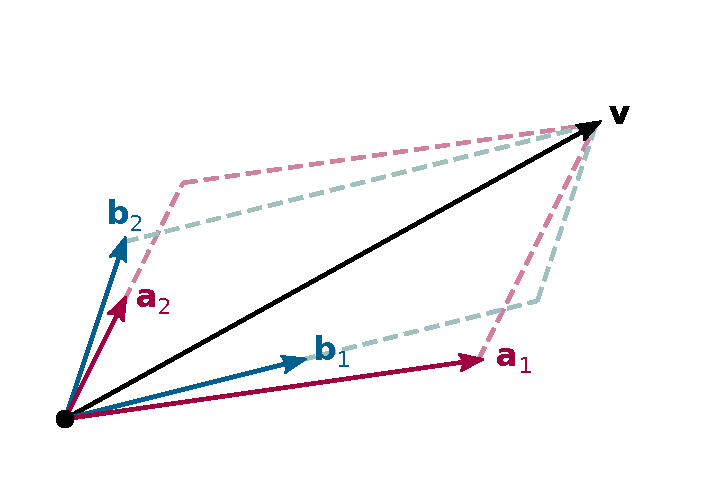
\includegraphics[width=72mm]{img/Abstrakt-in-Basis-BA.pdf}
\end{center}
\end{frame}

\begin{frame}
Was allerdings existiert, ist die Matrix
\[T_A^B := A^{-1}B.\]\pause
Diese Matrix nennen wir \emph{Transformationsmatrix}. Sie wandelt die
Koordinaten von $\bv v$ bezüglich Basis $B$ in die Koordinaten
bezüglich Basis $A$ um.\pause

\vspace{0.8em}
Als Formel:
\[\bv v_A = T_A^B \bv v_B.\]
\end{frame}

\begin{frame}
Wie bekommt man nun aber die Transformationsmatrix, wenn nur
eine Beziehung zwischen den Basisvektoren vorliegt? Gegeben sei
die Beziehung
\begin{align*}
\bv a_1 &= s_{11}\bv b_1 + s_{21}\bv b_2,\\
\bv a_2 &= s_{12}\bv b_1 + s_{22}\bv b_2.
\end{align*}\pause
Dies lässt sich in Kurzform schreiben als
\[\bv a_i = \sum_{j=1}^2 s_{ji}\bv b_j.\]
\end{frame}

\begin{frame}
Betrachten wir zur Hilfe kurz noch einmal den $\R^2$.\\
Da muss gelten
\[a_{ki} = \sum_{j=1}^2 s_{ji}b_{kj}.\]\pause
Na das ist doch eine Matrizenmultiplikation. Nämlich
\[A^T = S^T B^T\]
mit
\[S = \begin{pmatrix}s_{11} & s_{12}\\
s_{21} & s_{22}\end{pmatrix}.\]
\end{frame}

\begin{frame}
\strong{Jetzt kommt Matrizenrechnung zur Anwendung.}\pause

\vspace{1em}
Transposition auf beiden Seiten der Gleichung bringt
\[A = (S^T B^T)^T = BS.\]\pause
Infolge gilt $A^{-1} = S^{-1} B^{-1}$, und somit
$A^{-1}B = S^{-1}.$\pause

\vspace{1em}
Schließlich haben wir $T_A^B=S^{-1}$. Und dies ist auch wieder
im abstrakten Vektorraum gültig.
\end{frame}

\begin{frame}
Umgekehrt ist mit dieser Einsicht die Beziehung für das betrachtete
Beispiel ermittelbar. Es gilt
\[S = (A^{-1}B)^{-1} = B^{-1}A.\]\pause
Das macht
\[S = \begin{pmatrix}4 & 1\\ 1 & 3\end{pmatrix}^{-1}
\begin{pmatrix}7 & 1\\ 1 & 2\end{pmatrix}
= \tfrac{1}{11}\begin{pmatrix}20 & 1\\ -3 & 7\end{pmatrix}.\]
Konkret ist
\begin{align*}
\bv a_1 &= \tfrac{20}{11}\bv b_1 - \tfrac{3}{11}\bv b_2,\\
\bv a_2 &= \tfrac{1}{11}\bv b_1 + \tfrac{7}{11}\bv b_2.
\end{align*}
\end{frame}

\begin{frame}
\strong{Bemerkung.} Für eine beliebige Matrix
\[B = \begin{pmatrix}b_{11} & b_{12}\\ b_{21} & b_{22}\end{pmatrix}\]
mit $0\ne \det(B) = b_{11}b_{22}-b_{12}b_{21}$ gibt es die Formel
\[B^{-1} = \frac{1}{\det(B)}\begin{pmatrix}
 b_{22} & -b_{12}\\
-b_{21} &  b_{11}
\end{pmatrix}.\]
\end{frame}

\begin{frame}
Ende.
\vfill\hfill\modest{Juli 2020}\\
\hfill\modest{Creative Commons CC0 1.0}
\end{frame}


\end{document}


